\documentclass{standalone}
\usepackage{tikz}
\usepackage{pgfplots}

\begin{document}
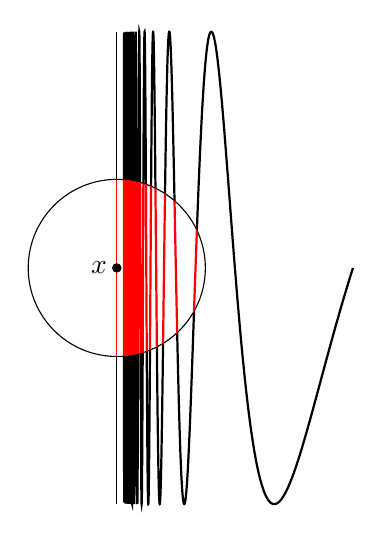
\begin{tikzpicture}[x=3cm, y=3cm]
\draw (0,-1) -- (0,1);
   % \draw[->] (0,-1) -- (0,1.1) node[above] {$\sin (1/x)$};
 \draw[domain=0.03:1,samples=5000, smooth, thick] plot (\x, {sin((pi/\x)r)});

  \filldraw[white] (0, 0) circle (31.7pt);
  \draw (0, 0) circle (32pt);
	\begin{scope}
	\clip (0, 0) circle (32 pt);
	\draw[red, domain=0.03:1,samples=5000, smooth, thick] plot (\x, {sin((pi/\x)r)});
	\draw[red] (0,-2) -- (0,2);
	\end{scope}
\filldraw (0, 0) circle (1.5pt) node[black, left] {$x$};
\end{tikzpicture}

\end{document}